%!TEX TS-program = xelatex
\documentclass[]{friggeri-cv}
\usepackage{afterpage}
\usepackage{hyperref}
\usepackage{color}
\usepackage{xcolor}
\hypersetup{
    pdftitle={},
    pdfauthor={},
    pdfsubject={},
    pdfkeywords={},
    colorlinks=false,       % no lik border color
   allbordercolors=white    % white border color for all
}
\addbibresource{bibliography.bib}
\RequirePackage{xcolor}
\definecolor{pblue}{HTML}{0395DE}

\begin{document}
\header{Arshpreet}     {Singh}
      {Software Engineer/Data Scientist}
      
% Fake text to add separator      
\fcolorbox{white}{gray}{\parbox{\dimexpr\textwidth-2\fboxsep-2\fboxrule}{%
.....
}}

% In the aside, each new line forces a line break
\begin{aside}
  \section{Address}
    3159, Sec-40D
    Chandigarh,Punjab, India
    ~
  \section{Tel \& LinkedIn}
    +91 991 5959387
    \href{http://www.linkedin.com/in/arsh840/}{www.linkedin\\.com/in/arsh840/}
    ~
  \section{Mail}
    \href{mailto:arsh840@gmail.com}{\textbf{arsh840@}\\gmail.com}
    ~
  \section{Web \& Git}
    \href{http://www.arshpreetsingh.wordpress.com}{arshpreetsingh.wordpress\\.com}
    \href{https://github.com/arshpreetsingh}{github.com/arshpreet\\singh}
    ~
  \section{Programming}
    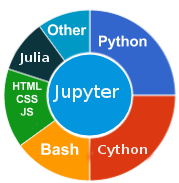
\includegraphics[scale=0.62]{img/programming.png}
    ~
  \section{OS Preference}
    \textbf{GNU/Linux}
\includegraphics[scale=0.40]{img/5stars.png}
    \textbf{Unix}
\includegraphics[scale=0.40]{img/5stars.png}
    \textbf{MacOS}
\includegraphics[scale=0.40]{img/2stars.png}
    \textbf{Windows}
\includegraphics[scale=0.40]{img/2stars.png}
    ~
  \section{Personal Skills}
    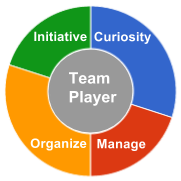
\includegraphics[scale=0.62]{img/personal.png}
    ~
\end{aside}

\section{Experience}
\begin{entrylist}
  \entry
    {01/12 - Now }
    {Freelance Developer \& Consultant}
    {Elance-Upwork/TCC GNDEC Ludhiana}
    {GNU/Linux software, LTSP Cluster implementation at PCTE(College for Technical Education) Baddowal,Ludhiana. Development of Flask-based Gmail Analyser show reports regarding Email Activity of company Employees,Rocks cluster(www.rockscluster.org) implementation and workshop at GNDEC Ludhiana, Development of advance volume filter using Paraview(www.paraview.org) and Python.}
  \entry
    {05/16 - 10/16}
    {Full-Stack Python Developer}
    {Revinfotech Ludhiana}
    {Design and development of Software Projects, Amazon and Google Cloud Management, LTSP implementation.Automation of various internal Tasks using Python, Project Management,Job hunting on Upwork.\\}
  \entry
    {01/13 - Now }
    {Administration and Management}
    {S.D. Sen. Sec. School,Barnala}
    {Transport and Quality management, Conduct various workshops to initiate programming and use of open source technologies, alongwith contributed to
Open-source projects. TuxMath, TuxPaint translation into Punjabi and Hindi languages,
Developed SDPS website, OpenStreet(www.osm.org) mapping done for 15
villages around SDPS, Implementation of LTSP(Linux terminal server project)
for computer-lab, Implemented Fedena(www.projectfedena.org) for School Management and ongoing development of Smart-Class project using
Raspberry-pie and Moodle.\\}
    \entry
    {01/14 - 02/15}
    {Linux Trainer and Web Developer}
    {FutureTech IT centre Ludhiana}
    {Teaching Linux Desktop and Server Administration skills to students. Devel-
oped various projects using technologies HTML, CSS, JavaScript, Python,
C and shell Script. Computer technical support. Problem solving related to hardware, software and Operating Systems. Management of the internal Structure.\\}
    \entry
    {01/13 - 06/13}
    {Intern-ship}
    {SysInfocom, Chandigarh}
    {Training for Linux Desktop and Server Administration, management and migration of servers. Development of ”Python Battery Saver pack”(Python
Based). Learning and using Latex for creating reports and documents.\\}
    \entry
    {06/11 - 07/11}
    {Intern-ship}
    {TCC GNDEC Ludhiana}
    {Training for Python. Worked on college souvenir(Django Based Project).
SageMath Deployment on Server and introduced SageMath and it’s features
to Research Students. Open Source Technologies.\\}
\\
\\
\\
\end{entrylist}
\section{Education}
\begin{entrylist}
  \entry
    {2009 - 2013}
    {Bachelor's Degree in Information Technology}
    {GNDCE Ludhiana,Punjab,India}
    {Main subjects: Mathematics and Physics,C,C++,Java,Python,JavaScript, Network Operating Systems,Web Technologies, Database Administration, Software Development.\\
    \emph{Major Project: ”Automation for Testing and consultancy cell”(Django Based). Project development carried out during intern-ship period at Sysinfocom Chandigarh}\\}
  \entry
    {2007 - 2009}
    {Senoir Secondary School}
    {DC Model, Ferozepur}
    {Main subjects: Mathematics, Physics, Chemistry.}
\end{entrylist}

\section{Certifications}
\begin{entrylist}
  \entry
    {12/2016}
    {Python for DataScience and Machine Learning}
    {Udemy. E-learning}
    {\emph{Pridiction of Stock Prices using Liner Regression}}
    
\end{entrylist}

\newpage

\begin{aside}
~
~
~
   \section{Languages}
    \textbf{English}
\includegraphics[scale=0.40]{img/4stars.png}
    \textbf{Hindi}
\includegraphics[scale=0.40]{img/5stars.png}
    \textbf{Punjabi}
\includegraphics[scale=0.40]{img/5stars.png}  
\end{aside}

\section{Projects}
\begin{entrylist} 
 \entry
    {03/2017}
    {Stock prediction using Random Forest}
    {Trading-Algorithm}
    {\emph{www.quantopian.com is used as platform to deploy,benchmark and evaluate performace of the Algorithm for
    single stock.}}
 \entry
    {01/2017}
    {Stock's Analysis using Ensemble Learning}
    {Research work}
    {\emph{Problem Definition: To Predict if close price of day N will be less or more than Close Price of Day N-1.
          Technologies Used: Python, Pandas, Numpy, Matplotlib, Scikit-learn.
          Features Used: Adj. Close, Daily Returns,Rolling Mean, Time-lagged series.}}
 \entry
    {08/2016}
    {Bitcoin Live Trading using ANN}
    {Revinfotech Ludhiana}
    {\emph{Bitcoin Live Trading is Web-Based System developed Using Django
    Framework. It uses Bitfinex Python API to produce Buy and Sell(Bitcoins Trading) calls
    as decided by Trading Strategy developed using ANN(Artificial Neural Network)}}
  \entry
    {12/2015}
    {Gmail Analyser}
    {Elance/Upwork}
    {\emph{Gmail Analyser is Flask Based Solution which provides data of All Emails
as per the request. Application is integrated with Gmail-Oauth2 login, pygal
python library is used to generate graphs based on Data, Whole application
is bootstrapped and optimised for mobile devices.}}
  \entry
    {03/2016}
    {ParaView Advanced Volume Filter}
    {Elance/Upwork}
    {\emph{ParaView is an open-source, multi-platform data analysis and visualization
application.Advanced Volume Filter
is developed using fsolve() function from scipy(Scientific Python) to find out
Volume intersection between two or more shapes.}}
 \entry
    {10/2013}
    {Centre-Table Design using OpenScad Scripting}
    {TCC GNDEC}
    {\emph{OpenScad is first C programming based CAD software which is used by var-
ious technologies those includes 3D printing and simulation. Centre table is
designed using Scripting language of OpenScad}}
 \entry
    {06/2012}
    {Battery Saver}
    {TCC GNDEC}
    {\emph{Battery Saver is responsible for keeping battery power between 40-80 per-
centage. A laptop battery could be prolonged by lowering the charge voltage
when connected to the AC grid. To make this feature user-friendly, a device
should feature a “Long Life” mode that keeps the battery at 4.05V/cell and
offers a capacity of about 80 percent. One hour before traveling, the user
requests the full Capacity mode to bring the charge to 4.20V/cell.}}
\end{entrylist}

\section{Open-Source Contributions}
\begin{entrylist}
 \entry
    {03/2016}
    {Tuxblocks}
    {Github}
    {\emph{Tuxblocks Game is developed to teach Algebra to School students using play-
ful method. Game is developed using Java Based PlayN Game Engine.
Hindi+Punjabi Translation of Game, Fixes for font-Class, Implementation of
Language translation system, Bug reports.}}

 \entry
    {03/2016}
    {Open Street Mapping}
    {osm.org}
    {\emph{Completed Digital mapping of 20 villages around my Village Kutba.}}

 \entry
    {03/2016}
    {Browser-Based File-Manager}
    {Github}
    {\emph{Flask based file manager, Contribution made to read/access any kind of
file(audio/video/images) whatever browser can support.}}

 \entry
    {03/2016}
    {Text-to-mp3 Android implementation}
    {Github}
    {\emph{Contributed to Open-source project Plyer by creating Python wrapper around
Java Classes.}}

      
\end{entrylist}


\\
\begin{flushleft}
\emph{March 11th, 2017}
\end{flushleft}
\begin{flushright}
\emph{Arshpreet singh Khangura}
\end{flushright}
\end{document}
